\chapter{Valutazione}

L'obiettivo del presente capitolo è discutere i risultati finora ottenuti, in particolare sulla base dei requisiti già soddisfatti e delle migliorie introdotte dal nuovo sistema rispetto alla versione legacy. Poiché il sistema è ancora in fase di sviluppo, non è possibile fornire una valutazione complessiva, effettuare un confronto esaustivo con il vecchio sistema, né presentare risultati di test prestazionali e di usabilità. Tuttavia, è possibile analizzare le funzionalità già progettate ed implementate, valutandone il contributo rispetto agli obiettivi iniziali e identificando le garanzie che il nuovo sistema è già in grado di fornire.

\section{Requisiti soddisfatti}
Sin dall'inizio era stato stabilito che questa tesi non avrebbe condotto alla realizzazione completa del sistema, ma si sarebbe concentrata principalmente sulle fondamentali fasi di analisi e progettazione, includendo anche l'implementazione di una prima versione funzionale. Nonostante ciò, è possibile tracciare un bilancio dei requisiti già soddisfatti, i quali evidenziano le potenzialità del nuovo sistema rispetto al precedente. A tal fine, i requisiti verranno suddivisi in due categorie: quelli già soddisfatti sia dal punto di vista progettuale che implementativo e quelli attualmente soddisfatti solo dal punto di vista progettuale.

\subsection{Elementi progettati e implementati}
Tra i requisiti soddisfatti, alcuni non si limitano alla fase di progettazione ma sono già stati concretamente implementati, costituendo il nucleo della prima versione del sistema. Questi elementi forniscono un primo miglioramento rispetto al legacy e rappresentano una base solida per l’evoluzione futura del progetto. Di seguito vengono analizzate le funzionalità già operative, evidenziandone l'impatto e le garanzie offerte.

\subsubsection{Dashboard panoramica per MSP e Dealer}
La prima funzionalità significativa già implementata è la dashboard panoramica, progettata specificamente per MSP e Dealer. Nel sistema legacy, questi utenti non disponevano di una visione aggregata ed efficace dei clienti sotto la loro gestione. Il nuovo sistema, invece, include una schermata con statistiche e grafici che permettono di ottenere una panoramica dettagliata delle attività del filtro DNS. In particolare, la dashboard mostra le seguenti informazioni:

\begin{itemize}
  \item Nella parte superiore, vengono presentate statistiche di base relative alle richieste elaborate dal filtro. Tra queste: il numero totale di richieste ricevute, il numero di minacce bloccate, il numero di categorie e indirizzi IP bloccati, il numero di categorie consentite, il numero di richieste DNS non risolte (NXDOMAIN) e, infine, il numero di richieste che hanno forzato l’utilizzo della SafeSearch sui motori di ricerca e YouTube. Questi dati offrono un quadro generale sul funzionamento del sistema e sull'efficacia del filtraggio.

  \item Nella parte centrale, sono presenti grafici per monitorare l’andamento delle richieste DNS. In particolare, vi è:
    \begin{itemize}
      \item Un grafico a barre che mostra le cinque categorie più bloccate;
      \item Un grafico a torta che rappresenta la distribuzione percentuale delle richieste DNS in base alla loro tipologia (richieste bloccate, richieste consentite, blocchi per IP, domini non risolti).
    \end{itemize}

  \item Nella parte inferiore, è presente un grafico che mostra l’andamento delle richieste DNS nel tempo, distinguendo tra quelle bloccate e quelle consentite.

  \item Tutti e tre i grafici consentono di modificare l'intervallo temporale di visualizzazione, permettendo di analizzare i dati su finestre temporali di 24, 48 o 72 ore.
\end{itemize}
%
Oltre a offrire una panoramica complessiva, la dashboard consente di visualizzare statistiche e report specifici per ciascun cliente gestito dall’MSP o dal Dealer. È infatti possibile selezionare un cliente dall'apposito menu a tendina e ottenere un quadro dettagliato delle sue attività. Questa funzionalità risulta particolarmente utile per monitorare eventuali anomalie o problemi specifici di un singolo cliente.

Al momento, la dashboard è ancora in una fase iniziale e non è possibile esprimere garanzie sulla qualità dell'aggregazione dei dati, che verrà affinata con le iterazioni successive dello sviluppo.

\begin{figure}
  \centering
  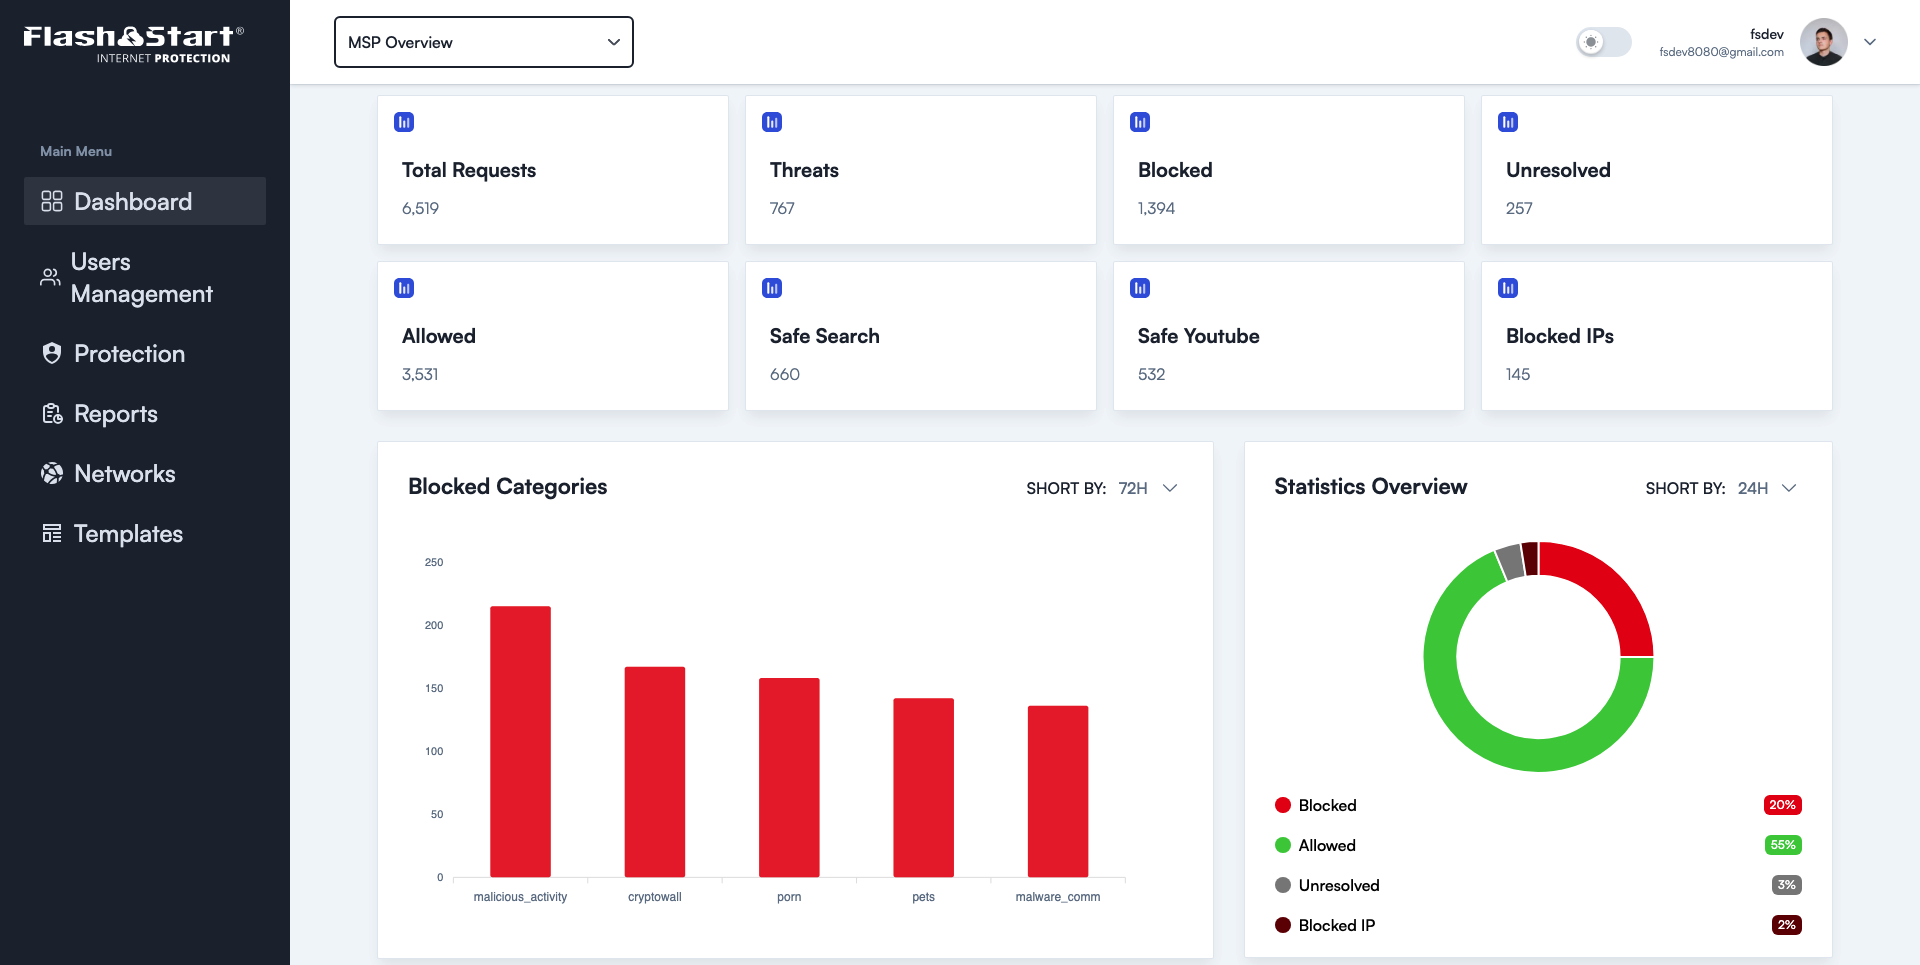
\includegraphics[width=1\textwidth]{figures/new-dashboard.png}
  \caption{Schermata del nuovo sistema che rappresenta la dashboard MSP.}
  \label{fig:dashboard-msp}
\end{figure}

\paragraph{Struttura e layout della dashboard}
Dal punto di vista dell’interfaccia utente, come si può vedere in \Cref{fig:dashboard-msp}, la dashboard è stata progettata con una struttura chiara e organizzata per garantire un’esperienza di navigazione fluida. Il menu di navigazione, posizionato nella parte sinistra dello schermo, è sempre visibile indipendentemente dalla pagina in cui ci si trova. Nei dispositivi aventi un display ridotto, come gli smartphone, il menu rimane nascosto per ottimizzare lo spazio e può essere aperto su richiesta dall’utente.

Nella parte superiore dell’interfaccia sono presenti diversi elementi chiave:
\begin{itemize}
  \item \textbf{Il logo dell'azienda}, posizionato a sinistra.
  \item \textbf{Il selettore del cliente}, che consente agli MSP di filtrare i report per un cliente specifico, oppure di lasciare l’opzione predefinita per visualizzare la panoramica di tutti i clienti gestiti.
  \item \textbf{Il selettore del tema}, situato sulla destra, che permette di passare dalla modalità scura a quella chiara.
  \item \textbf{L’area utente autenticato}, da cui è possibile accedere alle impostazioni del profilo e alla funzione di logout.
\end{itemize}
%
In futuro, nell’header verrà integrata una sezione notifiche, accessibile tramite un’icona che indicherà la presenza di nuovi avvisi e permetterà di visualizzarli all’interno di un pannello dedicato.

Infine, il corpo centrale della dashboard ospita i grafici e le statistiche descritte in precedenza, fornendo un’analisi dettagliata del traffico DNS e della sicurezza del sistema. L’interfaccia è stata progettata per garantire flessibilità, con un layout adattivo che ottimizza la visualizzazione su schermi di diverse dimensioni.

\subsubsection{Gestione della multiutenza}
La necessità di introdurre un sistema che supportasse la multiutenza ha costituito uno dei principali requisiti per il nuovo pannello. Rispetto al precedente, in cui la gestione degli account risultava assai limitata, la nuova implementazione permette ora di associare più credenziali di accesso a una singola organizzazione e di abilitare operazioni di creazione, modifica ed eliminazione degli utenti. Questa flessibilità si traduce in un notevole progresso rispetto al passato, consentendo a più persone, con diversi ruoli, di accedere alla dashboard e monitorare le informazioni di loro competenza.

Un ulteriore aspetto riguarda la futura integrazione del controllo degli accessi: sebbene tale meccanismo non sia ancora stato sviluppato, l’architettura del sistema è stata progettata per accogliere in modo agevole e graduale soluzioni di autorizzazione avanzate, basate su ruoli e permessi granulari. In questo modo, sarà possibile estendere ulteriormente la sicurezza e la modularità del pannello.

Sul fronte della protezione delle credenziali di accesso, è stato adottato l’algoritmo di hashing \texttt{bcrypt}. Quest’ultimo offre non solo una maggiore sicurezza contro attacchi di forza bruta, ma consente anche di aumentare il costo computazionale dell’hashing nel tempo, adeguandone la resistenza alla continua crescita della potenza di calcolo. In questo modo, il sistema può mantenere un elevato livello di protezione delle password anche sul lungo termine.

Per consentire una gestione semplice e immediata della multiutenza, è stata sviluppata un’apposita interfaccia che permette di inserire, aggiornare o rimuovere gli account, oltre che di assegnare ad ogni utente un ruolo specifico all’interno dell’organizzazione. Tale funzionalità costituisce le fondamenta su cui verrà costruito in futuro un sistema di controllo degli accessi più sofisticato, in grado di differenziare i privilegi sulle singole risorse applicative.

Nella \Cref{fig:user-management} viene mostrata la schermata dedicata alla gestione degli utenti, in cui è possibile osservare le form per l’inserimento, la modifica e l’eliminazione degli account.

\begin{figure}
  \centering
  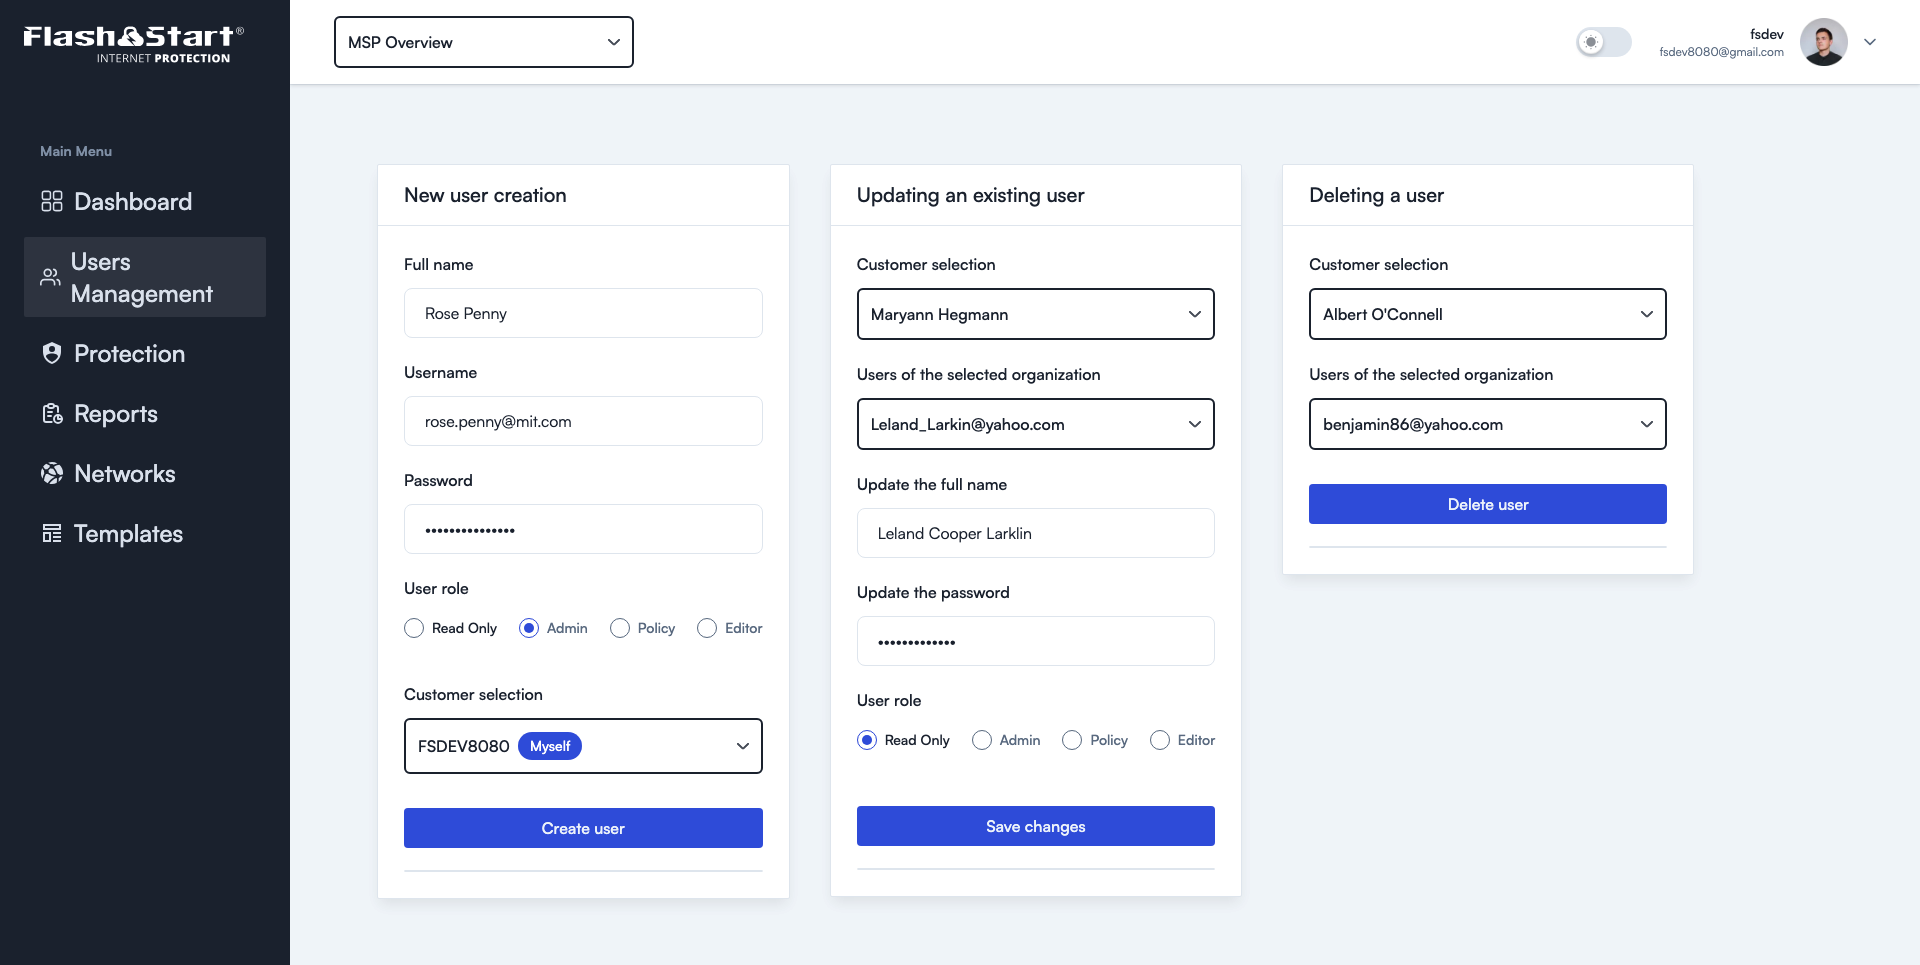
\includegraphics[width=1\textwidth]{figures/new-user-panel.png}
  \caption{Schermata del nuovo sistema per la gestione degli utenti.}
  \label{fig:user-management}
\end{figure}

\subsubsection{Supporto multilingua}
Un ulteriore requisito già soddisfatto è il supporto multilingua. Il frontend del nuovo sistema, infatti, possiede già il supporto completo alle lingue italiano e inglese. Sebbene possa sembrare un dettaglio secondario, questa funzionalità è fondamentale per un prodotto destinato a un mercato internazionale, in cui gli utenti parlano lingue diverse. Inoltre, l’architettura progettata consente di aggiungere nuove lingue in modo semplice, senza necessità di modifiche al codice sorgente, ma solo integrando nuovi file di traduzione.

\subsubsection{Gestione avanzata degli errori}
Un altro elemento progettato e implementato è la gestione avanzata degli errori, che introduce una strategia scalabile e strutturata per il trattamento delle anomalie sia lato backend che frontend.
%
Questa architettura garantisce diversi vantaggi:
\begin{itemize}
  \item \textbf{Robustezza e controllo a tutti i livelli del sistema}: la gestione degli errori è strutturata in modo gerarchico, coprendo dalla validazione degli input nelle API fino ai problemi a livello di database, evitando che errori non gestiti possano propagarsi in modo incontrollato.
  \item \textbf{Standardizzazione e interoperabilità}: gli errori vengono generati in modo schematizzato e dinamico, garantendo una rappresentazione uniforme e facilmente interpretabile da qualsiasi componente del sistema, sia interno che esterno.
  \item \textbf{Compatibilità con il sistema multilingua}: grazie alla struttura modulare degli errori, il frontend può costruire dinamicamente messaggi testuali in più lingue, senza dipendere da stringhe fisse predefinite nel backend.
  \item \textbf{Affidabilità del codice grazie a TypeScript}: il sistema di gestione degli errori sfrutta la tipizzazione statica di TypeScript, garantendo una maggiore sicurezza nella gestione delle eccezioni e facilitando l’individuazione di problemi già in fase di sviluppo.
\end{itemize}

Rispetto al sistema legacy, che gestiva gli errori in modo frammentato e poco strutturato, questa soluzione garantisce una maggiore affidabilità complessiva, riducendo il rischio di comportamenti inattesi e migliorando la manutenibilità del codice. Inoltre, la sua scalabilità consente di adattarlo facilmente a nuove esigenze, rappresentando un elemento chiave per la futura evoluzione del sistema.

\subsection{Elementi solo progettati}
In aggiunta alle funzionalità già realizzate, si evidenzia l’esistenza di alcuni aspetti che, sebbene non ancora sviluppati in maniera operativa, risultano già completamente definiti dal punto di vista progettuale. Nonostante la loro efficacia pratica non sia al momento valutabile, è comunque possibile analizzare il potenziale e il valore aggiunto che tali elementi apporteranno rispetto al sistema legacy.

\subsubsection{Gestione dei profili condivisi}
Uno degli elementi più significativi in questa categoria è l’introduzione dei profili condivisi. Questa novità consente di creare profili di protezione condivisibili tra più organizzazioni all'interno della stessa gerarchia. Essi possono essere visti come template di protezione, utili soprattutto per gli MSP e per i Dealer, che potranno così offrire configurazioni standardizzate e omogenee ai loro clienti.

Un altro vantaggio di questa funzionalità è la semplificazione della gestione della protezione: eventuali modifiche a un profilo condiviso vengono automaticamente propagate a tutte le organizzazioni che lo utilizzano. Questo rappresenta un miglioramento significativo rispetto al vecchio sistema, dove le configurazioni erano gestite separatamente per ogni organizzazione, con difficoltà nella loro manutenzione e uniformità.

L’introduzione dei profili condivisi permette inoltre al sistema di allinearsi con i competitor, alcuni dei quali già dispongono di questa funzionalità. Benché tale caratteristica non sia ancora implementata, la sua progettazione dettagliata consente di avere una chiara roadmap per la sua realizzazione e integrazione futura.

\subsubsection{Riprogettazione del database}
Il design della funzionalità appena descritta rientra in un più ampio processo di rimodellazione del database, che garantisce maggiore scalabilità e coerenza dei dati. Inoltre, la nuova struttura permette l’implementazione di funzionalità avanzate che il vecchio database, per sua natura, non poteva supportare. Questa revisione assicura che il sistema possa evolversi senza le limitazioni strutturali della versione legacy, rendendolo più flessibile, scalabile e adatto alle esigenze future.

Per quanto la riprogettazione del database sia stata completata principalmente a livello di schema concettuale, alcune componenti essenziali risultano già integrate nel sistema. In particolare, le nuove tabelle dedicate alla gestione degli utenti e delle organizzazioni sono già operative e costituiscono la base su cui si fonda il meccanismo di multiutenza. Queste modifiche hanno consentito di superare i vincoli del vecchio modello, che non era stato concepito per supportare una gestione avanzata degli accessi e delle gerarchie organizzative.

L’adozione del nuovo schema dati non solo migliora la struttura e la leggibilità del database, ma assicura anche una maggiore coerenza e manutenibilità, agevolando l’implementazione futura di altre funzionalità chiave. Inoltre, grazie al suo design modulare e scalabile, il database può adattarsi con facilità a nuove esigenze, garantendo flessibilità operativa e una gestione più efficiente dei dati.

\section{Miglioramenti pianificati}
Malgrado il nuovo sistema abbia già introdotto numerosi miglioramenti rispetto alla versione legacy, vi sono ancora diverse aree che non risultano complete, così come altre funzionalità che devono essere introdotte ex novo per garantire un'esperienza conforme alle esigenze operative previste. Tutti i punti trattati in questa sezione rappresentano miglioramenti già pianificati o previsti nella roadmap di sviluppo e verranno implementati nelle fasi successive rispetto a questa tesi.

\subsection{Gestione avanzata dei permessi e autenticazione}
L’attuale implementazione della multiutenza consente la creazione e la gestione di account con differenti ruoli, tuttavia, il controllo degli accessi richiede ulteriori sviluppi. In particolare, è prevista l’integrazione di un sistema \textit{Role-Based Access Control} per la gestione dei ruoli utente, combinato con un livello di autorizzazione che regoli i permessi legati all’organizzazione di appartenenza e alle licenze attive.

Per garantire un sistema di permessi strutturato ed efficace, sarà necessaria un’analisi approfondita per individuare tutte le operazioni da regolamentare e codificare in una tabella del database. Successivamente, il sistema dovrà essere integrato a tutti i livelli della piattaforma, assicurando un controllo uniforme sugli endpoint dell’API e sulle rotte del frontend.

In aggiunta, per migliorare ulteriormente la sicurezza e conformarsi agli standard più recenti, è prevista l’implementazione di un sistema di autenticazione multifattore (MFA). Questo elemento è particolarmente richiesto dai clienti operanti in settori sensibili, dove la protezione degli accessi rappresenta un requisito imprescindibile.

\subsection{Integrazione della brand identity nel frontend}
Attualmente, il frontend del sistema è stato sviluppato con un focus sulle funzionalità, senza un’integrazione effettiva della nuova identità visiva dell'azienda. Nelle fasi successive, è già previsto il coinvolgimento del designer responsabile del rinnovamento dell'immagine aziendale, garantendo così un'interfaccia armonizzata con il design system dell'organizzazione. Sebbene questo aspetto non incida direttamente sulle funzionalità, riveste un ruolo cruciale per l’accettazione del prodotto da parte degli utenti finali, che devono percepirlo come un sistema moderno, affidabile e in linea con l’identità del brand.

\subsection{Implementazione della nuova struttura del database}
Come è già stato evidenziato, la riorganizzazione del database risulta già delineata sotto il profilo concettuale e, attualmente, è stata resa operativa soltanto la componente relativa alla gestione della multiutenza. Per le restanti sezioni, invece, è in corso la traduzione in un database di test.

Un elemento cruciale nella roadmap è la definizione di un processo di migrazione dei dati dal sistema legacy alla nuova base dati. Tale passaggio consentirà di validare fin da subito la coerenza e l’integrità delle nuove tabelle, garantendo al contempo la prosecuzione dello sviluppo sulla versione migliorata del database.

\subsection{Aumento della copertura dei test}
Attualmente, l’infrastruttura di testing del frontend è stata predisposta e resa operativa, ma non dispone ancora di specifiche definite per garantire una copertura adeguata. Tuttavia, la \textit{coverage} al 100\% del codice sorgente rappresenta un requisito fondamentale per garantire la stabilità e l’affidabilità del sistema, in quanto contribuisce a individuare e correggere eventuali anomalie prima del rilascio in produzione.
%
Per soddisfare questo requisito è necessario incrementare la copertura dei test automatizzati, con particolare attenzione ai componenti critici dell’interfaccia utente. Questo aspetto è già stato pianificato e verrà affrontato nelle prossime iterazioni dello sviluppo, al fine di consolidare la qualità del software e ridurre il rischio di regressioni.

\subsection{Implementazione delle funzionalità chiave}
Oltre ai miglioramenti tecnici e architetturali già discussi, il completamento della prima release del sistema richiede l’integrazione di alcune macrofunzionalità fondamentali per garantirne la piena operatività. In particolare, il sistema dovrà includere:
\begin{itemize}
  \item \textbf{Gestione della protezione}: interfacce e strumenti dedicati alla configurazione delle policy di filtraggio e sicurezza, con un'efficace integrazione dei profili condivisi.
  \item \textbf{Generazione e visualizzazione avanzata dei report}: estensione del modulo di reporting per offrire un’analisi più dettagliata rispetto ai dati attualmente disponibili nella dashboard panoramica, così come la possibilità di esportare i report in formati standard.
  \item \textbf{Analisi del traffico in tempo reale}: strumenti per il monitoraggio live delle richieste DNS, utili per una gestione più dinamica della sicurezza di rete. Dovrà essere inclusa una funzione di ricerca avanzata per filtrare e analizzare i dati in tempo reale.
  \item \textbf{Gestione degli Endpoint remoti}: integrazione del sistema con i dispositivi mobili dotati di \textit{ClientShield}, per consentirne la configurazione e il monitoraggio da parte dei gestori del filtro.
\end{itemize}

Il nuovo sistema è destinato a sostituire integralmente il precedente, ragion per cui dovrà integrare fin dalla prima release tutte le macrofunzionalità della versione legacy, garantendo continuità nell’erogazione dei servizi e nella gestione della protezione e del traffico DNS. L’implementazione di tali moduli, dunque, non costituisce un semplice avanzamento, bensì un requisito imprescindibile per assicurare una transizione senza compromessi tra il vecchio e il nuovo sistema.

\subsection{Scrittura della documentazione}
Un aspetto fondamentale per garantire la manutenibilità e l’adozione efficace del nuovo sistema è la creazione di una documentazione completa e strutturata. Questo processo coinvolge tre aree principali: la documentazione del codice, la formalizzazione delle API e la stesura di un manuale utente.

Per quanto riguarda il codice sorgente, è essenziale integrare commenti dettagliati nelle parti più rilevanti e articolate, al fine di agevolare la comprensione della codebase da parte di nuovi sviluppatori. La documentazione interna sarà redatta esclusivamente in inglese, seguendo le best practices per i progetti software con una possibile espansione internazionale.

Parallelamente, sarà necessario predisporre una documentazione formale delle API, che descriva in modo chiaro gli endpoint disponibili, i parametri accettati e i formati di risposta previsti. Questa documentazione sarà tradotta nelle principali lingue per garantire un facile accesso agli sviluppatori esterni e ai partner tecnologici.

Infine, la redazione di un manuale utente sarà essenziale per facilitare l’adozione del nuovo sistema sia da parte dei nuovi utenti sia di coloro che effettuano la transizione dal pannello legacy. Il manuale dovrà includere istruzioni dettagliate sulle funzionalità disponibili e sarà tradotto nelle principali lingue, garantendo un supporto chiaro e accessibile a un’utenza internazionale.

L’implementazione di un processo di documentazione strutturato contribuirà significativamente a migliorare l’esperienza degli sviluppatori e degli utenti, garantendo una maggiore efficienza nella gestione del sistema e una più rapida curva di apprendimento.
